\section{2026.3.3 Linear double covers and finite-dimensional genuine representations}

$G$ is a linear real reductive group, $\tilde{G}$ is a double cover of $G$.

\begin{thm}
  $\tilde{G}_{0}$ is a linear group (i.e. there is an injective homomorphism $\tilde{G}_0 \to \GL_n(\BR)$ for some $n$) equivalent to the existence of a finite-dimensional genuine representation of $\tilde{G}$.
\end{thm}


\begin{proof}


  If $\tilde{G}_0$ is a linear group, there are two possibilities:

  \begin{itemize}
    \item $ \varepsilon  \notin \tilde{G}_0$: then $\{ 1, \varepsilon\} \times \tilde{G}_0$ is a subgroup of $\tilde{G}$ with finite index, and it has a finite-dimensional representation such that $\varepsilon$ acts by $-1$, so we get a finite-dimensional genuine representation of $\tilde{G}$ by induction.
    \item $\varepsilon \in \tilde{G}_0$: denote $\tilde{G}_0$ by $H$, then $H = A \times {^{0}H}$ as a Nash group, and $^0H$ is also a linear group. So there is a closed embedding of Nash groups $^0H \hookrightarrow \GL_n(\BR)$ for some $n$ ($^0H$ has compact center), take Zariski closure of $^0H$ in $\GL_n(\BC)$ we get the complexification $^0H_{\BC}$ of $^0H$, there is an algebraic matrix coefficient of $^0H_{\BC}$ such that $\varepsilon$ acts on it by $-1$, and it generates a finite-dimensional genuine representation of $\tilde{G}$ by induction.
  \end{itemize}
  
  
  Conversely, if there is a finite-dimensional genuine representation of $\tilde{G}$, we also have two possibilities:
  \begin{itemize}
    \item $\varepsilon \notin \tilde{G}_0$: then $\tilde{G}_0 \to G$ is injective, since $G$ is a linear group, $\tilde{G}_0$ is also a linear group.
    \item $\varepsilon \in \tilde{G}_0$: then we can find a finite-dimensional representation $E_1$ of $\tilde{G}_0$ such that $\varepsilon$ acts by $-1$. We also have a finite-dimensional faithful representation $E_2$ of $G$, we can regard it as a representation of $\tilde{G}_0$ by pullback, and $\varepsilon$ acts trivially on $E_2$. So $E_1 \oplus E_2$ is a finite-dimensional faithful representation of $\tilde{G}_0$.
  \end{itemize}
\end{proof}


\begin{rk}
  After I have a sleep, I find that $\tilde{G}_0$ can be repleced by $\tilde{G}$ in this theorem, and the proof is even easier.
\end{rk}





\section{2026.3.21 Geometry of the flag variety of $\mathrm{SL}_2(\BC)$}

In this section, we illustrate the geometry of the flag variety of $\mathrm{SL}_2(\BC)$, which serve as a simple example for understanding more general phenomena. 


$K = \BC^*$ action has three orbits on $\BP^1(\BC)$: two closed orbits $\{0\}$ and $\{\infty\}$, and one open orbit $\BC^*$. The conormal bundle of the open orbit is the zero section, while the conormal bundle of the closed orbits are the cotangent fiber at $0$ and $\infty$ respectively. So we have three conormal bundles, which are all Lagrangian subvarieties in $T^*\BP^1(\BC)$.



\begin{center}
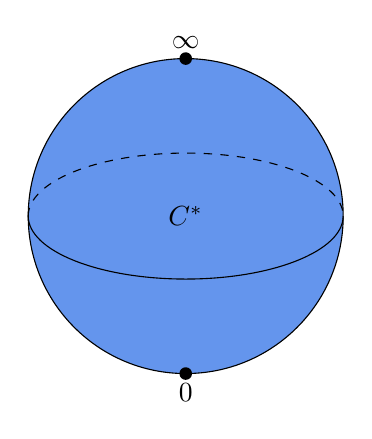
\begin{tikzpicture}[scale=2]

% Shade the open orbit C^*
\fill[CornflowerBlue] (0,0) circle (1);

% Draw sphere outline
\draw (0,0) circle (1);

% Draw equator
\draw (-1,0) arc (180:360:1 and 0.4);
\draw[dashed] (-1,0) arc (180:0:1 and 0.4);

% North pole (infinity)
\fill (0,1) circle (0.04);
\node[above] at (0,1) {$\infty$};

% South pole (0)
\fill (0,-1) circle (0.04);
\node[below] at (0,-1) {$0$};

% Label open orbit
\node at (0,0) {$\mathbb{C}^*$};

\end{tikzpicture}
\end{center}

For a $K$-equivariant perverse sheaf $\CF^{\bullet}$ on it, we calculate its characteristic cycle $\mathrm{CC}(\CF^{\bullet})$ use the formula

\[
\chi^{mic}_{S} = \sum_{S' > S} c(S,S') \chi^{loc}_{S'},
\]


only need to determine the coefficients $c(S,S') (= \sum_i (-1)^i H^i_c(J \cap S', K \cap S'; \BC))$ for $S' > S$, where $(J,K)$ is the normal Morse datum of S, which is well-defined up to homeomorphism.


\begin{itemize}
  \item For the open orbit $\BC^*$, we have $S' = \BC^*$ and $c(\BC^*,\BC^*) = -1$.
  \item For the closed orbit $\{0\}$, we have $S' = \{0\}, \BC^*$, and $c(\{0\},\{0\}) = 1$, for $c(\{0\},\BC^*)$, the pair $(J \cap S', K \cap S')$ is the following picture

\begin{center}
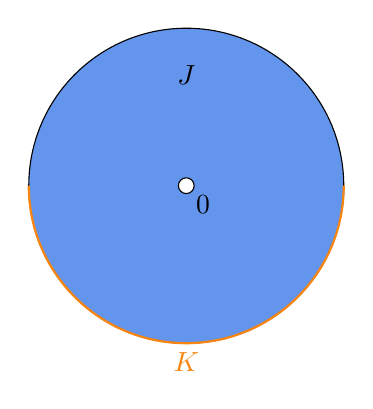
\begin{tikzpicture}[scale=2]

% Draw punctured disc (light fill)
\fill[CornflowerBlue] (0,0) circle (1);
\fill[white] (0,0) circle (0.05); % puncture at the origin

% Draw the boundary circle
\draw (0,0) circle (1);

% Draw the puncture as a hollow point
\draw (0,0) circle (0.05);
\node[below right] at (0,0) {$0$};

% Draw the lower half-cycle (closed subset K)
\draw[BurntOrange, thick] (1,0) arc (0:-180:1); % lower semicircle
\node[BurntOrange, below] at (0,-1) {$K$};

% Label the punctured disc
\node at (0,0.7) {$J$};

\end{tikzpicture}
\end{center}
therefore $c(\{0\},\BC^*) = \sum_i (-1)^i H^i_c(J \cap \BC^*, K \cap \BC^*; \BC) =^{?} -1$.
\end{itemize}


So we have

\begin{align*}
  \chi^{mic}_{0} &= \chi^{loc}_{0} - \chi^{loc}_{\BC^*}, \\ 
  \chi^{mic}_{\infty} &= \chi^{loc}_{\infty} - \chi^{loc}_{\BC^*}, \\
  \chi^{mic}_{\BC^*} &= -\chi^{loc}_{\BC^*}.
\end{align*}
 


\section{2026.3.22 Perverse sheaves on $\BC$}

Construuctible sheaves on $\BC = \BC^* \sqcup \{0\}$. Some calculations comes from the lecture notes by Geordie Williamson \cite{Wil15}.

Denote $j: \BC^* \hookrightarrow \BC$ the open inclusion, $i: \{0\} \hookrightarrow \BC$ the closed inclusion. Then we have the following six functors:
\[
\begin{tikzcd}[column sep=huge]
  D^b(\mathbb{C}^*) 
  \arrow[r, shift left=2.5ex, "j_!"]  
  \arrow[r, shift right=2.5ex, "j_*"'] 
  & D^b_c(\mathbb{C}) 
  \arrow[r, shift left=2.5ex, "i^*"] 
  \arrow[r, shift right=2.5ex, "i^!"']
  \arrow[l, "j^{*} = j^!" description] 
  & D^b(\{0\})
  \arrow[l, "i_* = i_!" description]
\end{tikzcd}
\]

$\CL$ is a local system on $\BC^*$. 

$j_!\CL$ has no quotient supported on $\{0\}$, $j_*$ has no subobject supported on $\{0\}$. $j_!\CL[1]$ and $j_*\CL[1]$ are perverse sheaves on $\BC$.


\begin{rk}
  Actually when $j: S \hookrightarrow  X$ is \colorbox{CornflowerBlue}{affine locally closed embedding} , $j_!$ and $j_*$ are $t$-exact for the perverse $t$-structure, so $j_!\CL[\dim S]$ and $j_*\CL[\dim S]$ are perverse sheaves on $X$.
\end{rk}
  



  



By easy calculation of group cohomology, we have:

\begin{align*}
  H^i(j_*\CL[1]_0) = \left\{
  \begin{array}{ll}
    0 & i \neq 0,-1 \\
    V_{\mu} & i = 0 \\
    V^{\mu} & i = -1
  \end{array}
  \right. 
\end{align*}

There is an exact sequence of perverse sheaves on $\BC$:
\[0 \to i_*V^{\mu} \to j_!\CL[1] \to j_*\CL[1] \to i_*V_{\mu} \to 0.\]






\section{2026.3.31 Enhanced flag variety and line bundles on $\CB$}
\noindent\textbf{\large I. The Enhanced Flag Variety and $G_0/N$ Isomorphism \cite{BB93}} 
\vspace{2mm}
\hrule 
\vspace{3mm}

$\fg$ be a complex semisimple Lie algebra, ${^{a}\fh} = \fb/[\fb,\fb]$ be the universal Cartan subalgebra, $G$ be the automorphism group of $\fg$, $G_0$ be the connected component of $G$, it is the adjoint group of $\fg$.

Attached to ${^{a}\fh}$ is a root system $\Delta$, and the Weyl group $W$. Although there isn't a well defined action of ${^{a}\fh} = \fb/[\fb,\fb]$ on $\fg/\fb = \fn^*$, the action of ${^{a}\fh}$ on $(\fn/[\fn,\fn])^*$ is well defined, and there is a canonical decomposition:
\[
  \left(\fn/[\fn,\fn]\right)^* = \bigoplus_{\alpha \in \Sigma} (\fn/[\fn,\fn])^*_{\alpha},
\]

Where $\Sigma$ is the set of simple roots. Note that this choice of positive root system is opposite to the one usually used in representation theory, but it is more natural in geometry since dominant implies positive line bundle in this way.

The enhanced flag variety $\tilde{\CB}$ is defined as the variety of pairs $(\fb, \{x_{\alpha}\}_{\alpha \in \Sigma})$ where $\fb$ is a Borel subalgebra of $\fg$, and $\xi$ is a nonzero element in $(\fn/[\fn,\fn])^*_{\alpha}$. There is a natural projection map $\pi : \tilde{\CB} \to \CB$ which forgets the second component, and is an $H$ principle bundle.

There is a $G$ action on $\tilde{\CB}$ defined by $g \cdot (\fb, \{x_{\alpha}\}_{\alpha \in \Sigma}) = (\Ad(g)\fb, \{\Ad^*(g)x_{\alpha}\}_{\alpha \in \Sigma})$. There is also an $H$ action on $\tilde{\CB}$ defined by $h \cdot (\fb, \{x_{\alpha}\}_{\alpha \in \Sigma}) = (\fb, \{\alpha(h)x_{\alpha}\}_{\alpha \in \Sigma})$. These two actions is compatible in the following way:
\[
  g \cdot h \cdot (\fb, \{x_{\alpha}\}_{\alpha \in \Sigma}) = \kappa_{g}(h) \cdot g \cdot (\fb, \{x_{\alpha}\}_{\alpha \in \Sigma}),
\]  

where $\kappa: G \to \mathrm{Aut}(H)$ is the action as outer automorphisms of $H$.

The adjoint group $G_0$ acts transitively on $\tilde{\CB}$, and the stabilizer of a base point $(\fb, \{x_{\alpha}\}_{\alpha \in \Sigma})$ is $N$. So we have an isomorphism $\tilde{\CB} \simeq G_0/N$. Under this identification, the $G$ action on $\tilde{\CB}$ is given by $g \cdot (g_0N) = gg_0(N)$, and the $H$ action on $\tilde{\CB}$ is given by $h \cdot (g_0N) = g_0 hN$.

\vspace{5mm}



\noindent\textbf{\large II. Line Bundles on $\CB$ and Very Ampleness}
\vspace{2mm}
\hrule 
\vspace{3mm}


Now $G$ is a connected reductive group.

\begin{lem}
  Let $G \to \GL(V)$ be a finite-dimensional representation of $G$, $k \cdot v \subseteq V$ be a one-dimensional subspace, $P = \mathrm{Stab}_G(k \cdot v)$. Suppose that $k_{\lambda}$ be the one-dimensional representation of $P$ defined by the action of $P$ on $k \cdot v$, then $i^*(\CO_{\BP(V)}(1)) = \CO_{G/P}(\lambda)$.
\end{lem}

\begin{proof}
  Note that $\CO_{\BP(V)}(-1)$ is the tautological line bundle, $P$ action on the fiber of $\CO_{\BP(V)}(-1)$ at $k \cdot v$ is given by $k_{\lambda}$. So $k_{-\lambda}$ for $\CO(1)$, also note that $\CO_{G/P}(\lambda) = G \times^{P} k_{-\lambda}$.
\end{proof}

\begin{lem}
  $\CO_{\CB}(\lambda)$ is very ample if and only if $\lambda$ is regular dominant ($\lambda \in X^+(H)$).
\end{lem}

\begin{proof}
  Consider the Verma module $V^{\lambda} = \CU(\fg) \otimes_{\CU(\fh)} k_{\lambda}$. By the transitive group action of $G$ on $\CB$, $\CO(\lambda)$ is generated by global sections $\Gamma(\CB,\CO(\lambda)) = V^{\lambda}$. Hence there is a surjection $\Gamma(\CB,\CO(\lambda)) \twoheadrightarrow \CO(\lambda) \otimes_k k_{eB} = k_{\lambda}$. Taking dual, we have $k_{-\lambda} \hookrightarrow (V^{\lambda})^*$.
  
  Since $\lambda$ is regular dominant, the stablizer of $k_{-\lambda}$ in $(V^{\lambda})^*$ is the Borel $B$, by the previous lemma, we have a $G$-equivariant morphism $\CB \hookrightarrow \BP((V^{\lambda})^*)$ such that $\CO(\lambda)$ is the pullback of $\CO(1)$, hence $\CO(\lambda)$ is very ample.
\end{proof}





\section{2026.4.5 Tangent map of the projection $G \times^P V \to V$}
$G$ is a compex algebraic group, $P$ is a closed subgroup of $G$ with a finite dimensional rational representation $V$. suppose that $\fg = \fu \oplus \fp$.

\[
  \begin{tikzcd}
    Y = G \times^P V \arrow[r, "\pi"] \arrow[d] & V \\
    G/P & 
  \end{tikzcd}
\]

There is an isomorphism:

\[
  \fu \oplus V \xrightarrow{\sim} T_{\bar{(1,\alpha)}}(G \times^P V)  ,
\]
which sends $(u,v)$ to $u^{\sharp} + v$, where $v \in V$ is regarded as a tangent vector of the fiber $V$ at $\alpha$, and $u^{\sharp}$ is the vector field on $Y$ generated by the action of $u \in \fu \subset \fg$.
 
The tangent map of $\pi$ at $\bar{(1,\alpha)}$ is:
\begin{align*}
  d \pi_{\bar{(1,\alpha)}} &: \fu \oplus V \to T_{\bar{(1,\alpha)}}(G \times^P V) \to V, \\
  d\pi_{\bar{(1,\alpha)}}(u,v) &= u \cdot \alpha + v,
\end{align*}
since $\pi(g,\alpha) = g \cdot \alpha$.

The above calculation is instrumental in extending the Kostant-Kirillov symplectic form of nilpotent orbits to the Jacobson-Morozov resolution of a nilpotent orbit:
\[
\begin{tikzcd}
  G \times^P \fg_{\geq 2} \arrow[r, "\pi"] & \bar{\BO} \\
  G \times^{P}  P \cdot e = G/Z_P(e) \arrow[r] \arrow[u,hookrightarrow ] & \BO \arrow[u,hookrightarrow ] 
\end{tikzcd}
\]

\[
  \pi^* \omega_{KK,\alpha}((u,v),(x,y)) = \kappa(\alpha, [u,x]) + \kappa(u,y) - \kappa(v,x).
\]
Where $(u,v), (x,y) \in \fg_{\leq -1} \oplus \fg_{\geq 2} = T_{\bar{(1,\alpha)}}(G \times^P \fg_{\geq 2})$.

This 2-form can be extended to a $G$-invariant 2-form $\omega_Y$ on $G \times^P \fg_{\geq 2}$. 

It is easy to check that $\mathrm{Rad}(\omega_{Y}) = \fg_{-1} \oplus 0$, so this form is symplectic if and only if $\fg_{-1} = 0$, which is equivalent to the nilpotent orbit $\BO$ is even.

\section{2026.4.22 Symplectic Form and Moment map}

\cite{Losev2022Topics}
\subsection{Examples of Symplectic Form and Moment map}

\begin{prop}
  The Kostant-Kirillov form $\omega_{KK}$ on a coadjoint orbit $\BO$ is closed and hence symplectic.
\end{prop}

\begin{proof}
  For $X \in \fg$ we have a vector field $X^{\sharp}$ on $\BO$ defined by 
  \[
    \boxed{\displaystyle X^{\sharp}_{\alpha} = \frac{\dd}{\dd t} \bigg|_{t=0} \Ad^*(\exp(tX))\alpha = [X,\alpha]}
  \]
  
  Define a smooth function $f_{X} = \kappa \bra{-,X}$ on $\BO$, then we have
  \[  \dd f_{X}(Y^{\sharp}) = \kappa([Y,\alpha],X) = \kappa(\alpha,[X,Y]) = \omega_{KK}(X^{\sharp},Y^{\sharp}). \]
  So $\iota_{X^{\sharp}} \omega_{KK} = df_{X}$.

  By Cartan's magic formula, we have
  \[  \CL_{X^{\sharp}} \omega_{KK} = \dd \iota_{X^{\sharp}} \omega_{KK} + \iota_{X^{\sharp}} \dd \omega_{KK} = \dd \dd f_{X} + \iota_{X^{\sharp}} \dd \omega_{KK} = \iota_{X^{\sharp}} \dd \omega_{KK}. \]
  Since $\omega_{KK}$ is $G$-invariant, $\CL_{X^{\sharp}} \omega_{KK} = 0$, hence $\iota_{X^{\sharp}} \dd \omega_{KK} = 0$ for all $X \in \fg$. Since the vector fields $X^{\sharp}$ span the tangent space of $\BO$ at each point, we have $\dd \omega_{KK} = 0$.
\end{proof}



Now, we cansider the simplest example of Hamiltonian $G$-space. 

Let $(V,\omega)$ be a complex symplectic space, and $G = \Sp(V,\omega)$

\begin{prop}
  The moment map $\mu : V \to \fg^*$ is given by $\bra{\mu(v),X} = \frac{1}{2}\omega(Xv,v)$ for $v \in V$ and $X \in \fg$.
\end{prop}

\begin{proof}
  Set $H_X(v) = \bra{\mu(v),X}$, we only need to check that $\iota_{X^{\sharp}} \omega = \dd H_X$:
  \begin{align*}
    (\dd H_X)_{v}(\delta v) &= \frac{1}{2} \omega(X \delta v, v) + \frac{1}{2} \omega(Xv, \delta v) \\
    &= \omega(Xv, \delta v) \\
    &= (\iota_{X^{\sharp}} \omega )_{v}(\delta v).
  \end{align*}
  Where $\delta v$ is a tangent vector of $V$ at $v$, which can be identified with an element in $V$ itself.
\end{proof}

\begin{rk}
  Note that $X^{\sharp}(v) = X \cdot v$ for $v \in V$.
\end{rk}

\begin{lem}
  The symplectic group $G$ acts transitively on $V \backslash \Bra{0}$.
\end{lem}

\begin{proof}
  Use induction on the dimension.
\end{proof}


\begin{prop}
  The moment map $\mu: V \backslash \Bra{0} \to \fg^*$ is a double cover onto the minimal nilpotent orbit $\BO_{min}$ in $\fg^*$.
\end{prop}

\begin{proof}
  Use trace form on $\fg$ to identify $\fg$ with $\fg^*$, then we can check that $\mu(v) = (u \mapsto \omega(v,u)v) \in \fg$.
  $\mu(v)$ is nilpotent since $\mu(v)^2 = 0$, and the image of $\mu$ is a nonzero nilpotent orbit. It is the minimal nilpotent orbit since $\mu(v)$ has rank $1$. $G$ acts transitively on $V \backslash \Bra{0}$, $\mu$ is a double cover onto $\BO_{min}$.
\end{proof}

\begin{rk}
  $\BO_{min} = \sqbra{2,1, \cdots,1}$ and $\pi_{1}^{G}(\BO_{\min}) = \BZ/2\BZ$, the cover above is the universial cover of $\BO_{min}$.
\end{rk}



\subsection{Classical and Quantum Fromal Darboux Theorems}

The classical Darboux theorem states that every point in a symplectic manifold has a neighborhood that is symplectomorphic to an open subset of the standard symplectic vector space. Here we investigate a formal algebraic analog of this theorem and its extension to quantization.

\begin{lem}
  Let $A$ be a Poisson algebra and $\fm$ be its maximal ideal with $A/\fm = \BC$. Then the Poisson bracket on $A$ induces a skew-symmetric form on $\fm/\fm^2$.
\end{lem}

\begin{proof}
  Define the skew-symmetric form as:
  \[
    \omega(a + \fm^2, b + \fm^2) = \{a,b\} \mod \fm.
  \]
\end{proof}

Now let $A = \mathbb{C}[[x_1, \dots, x_{2n}]]$ so that there is a unique maximal ideal $\fm = (x_1, \dots, x_{2n})$ and $\fm/\fm^2$ is spanned by $x_i + \fm^2$. Suppose that the Poisson bracket on $A$ induces a non-degenerate skew-symmetric form on $\fm/\fm^2$. So $\{x_i, x_j\} = \omega_{ij} \mod \fm$ for some $\omega_{ij} \in \BC$, then the matrix $(\omega_{ij})$ is non-degenerate skew symmetric.

\begin{thm}[Formal Darboux Theorem]
   There exists a formal change of coordinates $y_i = y_i(x_1, \dots, x_{2n}) \in \fm$ such that $\{y_i, y_j\} = \omega_{ij} \in \BC$.
\end{thm}

\begin{proof}
  Use induction, suppose that we have found $x_{i}^{\bra{n}} \in \fm$ such that $\Bra{x_{i}^{\bra{n}}, x_{j}^{\bra{n}}} \equiv \omega_{ij} \mod \fm^n$ (i.e. $\Bra{x_i^{(n)}, x_j^{(n)}} = \omega_{ij} + R_{ij}^{(n)} $ for some $R_{ij}^{(n)} \in \fm^n$). We want to find $\delta_i^{\bra{n}} \in \fm^{n+1}$ such that $\Bra{x_i^{\bra{n}} + \delta_i^{\bra{n}}, x_j^{\bra{n}} + \delta_j^{\bra{n}}} \equiv \omega_{ij} \mod \fm^{n+1}$.
  
  Since 
  \begin{align*}
    \Bra{x_i^{(n)} + \delta_i^{(n)}, x_j^{(n)} + \delta_j^{(n)}} &= \Bra{x_i^{(n)}, x_j^{(n)}} + \Bra{\delta_i^{(n)}, x_j^{(n)}} + \Bra{x_i^{(n)}, \delta_j^{(n)}} + \Bra{\delta_i^{(n)}, \delta_j^{(n)}} \\
    &\equiv \Bra{x_i^{(n)}, x_j^{(n)}} + \Bra{\delta_i^{(n)}, x_j^{(n)}} + \Bra{x_i^{(n)}, \delta_j^{(n)}} \mod \fm^{n+1}\\
    &\equiv \omega_{ij} + R_{ij}^{(n)} + \Bra{x_i^{(n)}, \delta_j^{(n)}} - \Bra{ x_j^{(n)}, \delta_i^{(n)}} \mod \fm^{n+1}.
  \end{align*}
  We need to solve the following equation for $\delta_i^{(n)}$:
  \[\Bra{x_i^{(n)}, \delta_j^{(n)}} - \Bra{ x_j^{(n)}, \delta_i^{(n)}} = -R_{ij}^{(n)} \mod \fm^{n+1}.\]
  
  Note that $\Bra{x_i^{(n)}, \delta_j^{(n)}} - \Bra{ x_j^{(n)}, \delta_i^{(n)}} = \omega_{ik}x_k^{(n)}\frac{\partial \delta_j^{(n)}}{\partial x_k} - \omega_{jk}x_k^{(n)}\frac{\partial \delta_i^{(n)}}{\partial x_k}$, we can solve the above equation by setting 
  $$\delta_i^{(n)} = -\frac{1}{n+1} \sum_{k,l} \omega^{kl} x_k^{(n)} R_{li}^{(n)}.$$
  
  Set $x_i^{(n+1)} = x_i^{(n)} + \delta_i^{(n)}$, then $y_i = \lim_{n \to \infty} x_i^{(n)}$ satisfies $\{y_i, y_j\} \in \BC$.
\end{proof}


\begin{thm}[Quantum Formal Darboux Theorem]
  Let $\CA_{\hbar}$ be a formal quantization of the Poisson algebra $A$. Then there are elements $\hat{y_i} \in \CA_{\hbar}$ such that
  \begin{itemize}
    \item $\hat{y_i} \equiv x_i \mod \hbar \CA_{\hbar}$;
    \item $\frac{1}{\hbar}\left[\hat{y_i}, \hat{y_j}\right] \in \BC$.
  \end{itemize}
\end{thm}

\begin{proof}
  Choose lift of $y_i$ in $\CA_{\hbar}$, denoted by $\hat{y_i}^{(1)}$. Then $\frac{1}{\hbar}\left[\hat{y_i}^{(1)}, \hat{y_j}^{(1)}\right] \equiv \{y_i, y_j\} = \omega_{ij} \mod \hbar$, so we can write $\frac{1}{\hbar}\left[\hat{y_i}^{(1)}, \hat{y_j}^{(1)}\right] = \omega_{ij} + \hbar R_{ij}^{(1)}$ for some $R_{ij}^{(1)} \in \CA_{\hbar}$ and $\omega_{ij} \in \BC$.

  Again, use induction, suppose that we have found $\hat{y}_i^{(n)}$ lift $y_i$ such that $\frac{1}{\hbar}\left[\hat{y}_i^{(n)}, \hat{y}_j^{(n)}\right] = \omega_{ij} + \hbar^{n} R_{ij}^{(n)}$ for some $R_{ij}^{(n)} \in \CA_{\hbar}$, we want to find $\delta_i^{(n)} \in \hbar^{n+1} \CA_{\hbar}$ such that $\frac{1}{\hbar}\left[\hat{y}_i^{(n)} + \delta_i^{(n)}, \hat{y}_j^{(n)} + \delta_j^{(n)}\right] = \omega_{ij} + \hbar^{n+1} R_{ij}^{(n+1)}$.

  This is equivalent to solving the following equation for $\delta_i^{(n)}$:
  \[\frac{1}{\hbar}\left[\hat{y}_i^{(n)}, \delta_j^{(n)}\right] - \frac{1}{\hbar}\left[\hat{y}_j^{(n)}, \delta_i^{(n)}\right] = -\hbar^{n} R_{ij}^{(n)} \mod \hbar^{n+1}.\]
  Note that $\frac{1}{\hbar}\left[\hat{y}_i^{(n)}, \delta_j^{(n)}\right] - \frac{1}{\hbar}\left[\hat{y}_j^{(n)}, \delta_i^{(n)}\right] = \omega_{ik} \hat{y}_k^{(n)}\frac{\partial \delta_j^{(n)}}{\partial \hat{y}_k} - \omega_{jk} \hat{y}_k^{(n)}\frac{\partial \delta_i^{(n)}}{\partial \hat{y}_k}$, we can solve the above equation by setting
$$\delta_i^{(n)} = -\frac{1}{n+1} \sum_{k,l} \omega^{kl} \hat{y}_k^{(n)} R_{li}^{(n)}.$$
  
  Set $\hat{y}_i^{(n+1)} = \hat{y}_i^{(n)} + \delta_i^{(n)}$, then $\hat{y}_i = \lim_{n \to \infty} \hat{y}_i^{(n)}$ satisfies $\frac{1}{\hbar}\left[\hat{y}_i, \hat{y}_j\right] = \omega_{ij} \in \BC$.
\end{proof}


\subsection{Localness of Differential Operators}

\aiblock{
  Any differential operator on $A$ can extend to localizations and completions.
  \begin{itemize}
    \item Extension to the Localization $S^{-1}A$. Let $A$ be a commutative algebra over a field $k$. A $k$-linear map $L: A \to A$ is a differential operator of order $\le k$ if for any $a_0, \dots, a_k \in A$, the iterated commutator vanishes:$$[\dots[[L, a_0], a_1], \dots, a_k] = 0$$where $[L, a](b) = L(ab) - aL(b)$. We denote the space of such operators as $\text{Diff}^k(A)$.The General Extension FormulaFor any $L \in \text{Diff}^k(A)$, the unique extension $\widetilde{L} \in \text{Diff}^k(S^{-1}A)$ is determined by its action on the reciprocal of an element $s \in S$. The formula uses the iterated adjoint action $\text{ad}_s(L) = [L, s]$:$$\widetilde{L}\left(\frac{1}{s}\right) = \sum_{j=0}^{k} (-1)^j s^{-(j+1)} \text{ad}_s^j(L)(1)$$Applying this to a general fraction $\frac{a}{s}$ via the Leibniz-like property for higher-order operators, we get:$$\widetilde{L}\left(\frac{a}{s}\right) = \sum_{j=0}^{k} (-1)^j s^{-(j+1)} \text{ad}_s^j(L)(a).$$
    \item Specific Cases for Low OrderOrder 0 (Multiplication by $f \in A$):$$\widetilde{L}\left(\frac{a}{s}\right) = s^{-1}(f \cdot a) = \frac{fa}{s}$$Order 1 (Derivations, where $L(1)=0$):Using the general formula for $j=0, 1$:$$\widetilde{L}\left(\frac{a}{s}\right) = s^{-1}L(a) - s^{-2}[L, s](a) = \frac{L(a)}{s} - \frac{L(sa) - sL(a)}{s^2} = \frac{sL(a) - aL(s)}{s^2}$$Order 2 (e.g., a Laplacian $\Delta$):$$\widetilde{L}\left(\frac{a}{s}\right) = \frac{\Delta(a)}{s} - \frac{\Delta(sa)-s\Delta(a)}{s^2} + \frac{\Delta(s^2 a) - 2s\Delta(sa) + s^2\Delta(a)}{s^3}.$$
    \item Extension to the Completion $\widehat{A}$. Let $I \subset A$ be an ideal. The completion is the inverse limit $\widehat{A} = \varprojlim A/I^n$.The Continuity PrecisionA differential operator $L$ of order $k$ is stricly continuous with respect to the $I$-adic topology because it satisfies:$$L(I^n) \subseteq I^{n-k} \quad \text{for all } n \ge k$$This filtration ensures that for any Cauchy sequence $(a_n)$ in $A$, the sequence $(L(a_n))$ is also Cauchy in the $I$-adic sense. The extension $\widehat{L}: \widehat{A} \to \widehat{A}$ is defined by taking the limit of the action on the truncated sequences:$$\widehat{L}\left( \lim_{n \to \infty} a_n \right) = \lim_{n \to \infty} L(a_n)$$Because $L$ is a polynomial-type operator (it "sees" only a finite neighborhood of any point algebraically), this limit is always well-defined and unique.
    \item The Poisson Bracket CaseA Poisson bracket $\{ \cdot, \cdot \}$ is a bilinear map that is a derivation (order 1 operator) in each slot.On $S^{-1}A$: Since $L_f = \{f, \cdot\}$ is a derivation, the extension is forced by the first-order formula derived above. For $a/s, b/t \in S^{-1}A$:$$\left\{ \frac{a}{s}, \frac{b}{t} \right\} = \frac{1}{s^2 t^2} \left( st\{a, b\} - at\{s, b\} - bs\{a, t\} + ab\{s, t\} \right)$$On $\widehat{A}$: Since the bracket is a derivation in each variable, it is continuous in each variable. By the universal property of completions of bilinear maps, it extends uniquely:$$\{ \hat{a}, \hat{b} \}_{\widehat{A}} = \lim_{n \to \infty} \{ a_n, b_n \}_A$$This ensures that $\widehat{A}$ inherits the Poisson algebra structure from $A$ without any ambiguity.
  \end{itemize}
  }





\section{2026.4.24 Normality of Nilpotent Orbits}

\textbf{Normality of Closure of Nilpotent Orbits}

\begin{thm}[Main theorem]
  For a nilpotent otbit $\BO$ in a complex semisimple Lie algebra $\fg$, its closure $\bar{\BO}$ is normal if and only if $\BC[\BO] = \BC[\bar{\BO}]$.
\end{thm}

\begin{lem}[Serre's criterion for normality]
  A is a commutative Noetherian ring. Then $A$ is normal if and only if it satisfies the following two conditions:
\begin{itemize}
  \item [($R_1$)] For any prime ideal $\fp$ of $A$ with $\mathrm{ht}(\fp) \leq 1$, the localization $A_{\fp}$ is a regular local ring.
  \item [($S_2$)] For any prime ideal $\fp$ of $A$, we have $\mathrm{depth}(A_{\fp}) \geq \min\{2, \mathrm{ht}(\fp)\}$.
\end{itemize}
\end{lem}

\begin{proof}[Proof of Main Theorem]
  ($\Rightarrow$) If $\bar{\BO}$ is normal, then by Serre's criterion, we get infromation about the depth inequality, and then we can apply the algebraic Hartogs theorem \cite[Chapter III, Exercise 3.5]{Har77} to conclude that $\BC[\BO] = \BC[\bar{\BO}]$.

  ($\Leftarrow$) If $\BC[\BO] = \BC[\bar{\BO}]$, then $\BC[\bar{\BO}]$ is a domain and integrally closed in its field of fractions, Since $\BC[\BO]$ is smooth. Hence $\BC[\bar{\BO}]$ is normal.
\end{proof}



\section{2026.4.25 Filtered Quantization of Nilcone}

\cite{Losev2022Topics}

\begin{lem}
  Let $A$ be a filtered algebra, $I \subseteq A$ an ideal, we have a short exact sequence:
  \[
    0 \to \gr I \to \gr A \to \gr (A/I) \to 0.
  \]
\end{lem}

\begin{proof}
  $I$ has an induced filtration $I_{\leq n} = I \cap A_{\leq n}$, and $\gr I = \bigoplus_{n} I_{\leq n}/I_{\leq n-1}$ is a graded ideal of $\gr A$. It is easy to see that the map $\gr A \to \gr (A/I)$ is surjective, and $\gr I \to \gr A$ is injective. For an element $a + A_{\leq i-1} \in \gr_{i} A$, then
  \begin{align*}
    &a + A_{\leq i-1} \mapsto 0 \in \gr_{i}(A/I) \\
    \Leftrightarrow \quad  &\bar{a} \in (A/I)_{\leq i-1} \\
    \Leftrightarrow \quad  &\exists \ a' \in A_{\leq i-1} \text{ such that } a - a' \in I \\
    \Leftrightarrow \quad  &a + A_{\leq i-1} \in I_{\leq i}/I_{\leq i-1}.
  \end{align*}
\end{proof}

\begin{rk}
  If $I = \langle f_1, \cdots , f_n\rangle$, then $\langle\sigma(f_1),\cdots,\sigma(f_n)\rangle \subseteq \gr I$.
\end{rk}  

\begin{prop}
  $A$ is a $\BZ_{\geq0}$ graded Noetherian Poisson algebra with $\deg \Bra{,} = -d < 0$, $\CA$ is its filtered quantization, and $\CI = \langle \hat{f_1}, \cdots, \hat{f_n}  \rangle$ ($\hat{f}_i \in \CA_{d_i}$), $f_i = \hat{F_i} + \CA_{\leq d_i -1}$, with the following conditions:
\begin{itemize} 
  \item $f_1, \cdots, f_n$ is a regular sequence in $A$;
  \item $\sqbra{\hat{f}_i, \hat{f}_j} = \sum_{i = 1}^{r} \hat{c}_{ij}^k \hat{f}_k$, with $\hat{c}_{ij}^k  \in \CA_{\leq d_i + d_j -d -d_k}$.
\end{itemize}
Then $\gr \CI = \langle f_1, \cdots, f_n\rangle$.
\end{prop}
  

\begin{proof}
  We only need to check that $\gr \CI \subseteq \langle f_1, \cdots, f_n\rangle$. Assume on the contrary that there exists a positive integer $e$ and $\hat{b}_i \in \CA_{\leq e-d_i}$ such that $\sigma(\sum_{i=1}^{n} \hat{b}_i \hat{f}_i) \notin \langle f_1, \cdots, f_n\rangle$. Also assume $e$ is the smallest integer with this property.
  
  Note that $\sum_{i=1}^{n} b_i f_i \in A_{e}$ must be zero, otherwise $\sigma(\sum_{i=1}^{n} \hat{b}_i \hat{f}_i) = \sum_{i=1}^{n} b_i f_i \in \langle f_1, \cdots, f_n\rangle$. So by the vanishing of the first Koszul homology, we can find $b_{ij} \in A$ such that $b_i = \sum_{j=1}^{n} b_{ij} f_j$ and $b_{ij} = -b_{ji}$ for $i \neq j$. By restriction to the degree $d_i$ we can assume that $b_{ij} \in A_{\leq e-d_i - d_j}$, take lifts $\hat{b}_{ij} \in \CA_{\leq e-d_i - d_j}$, such that $\hat{b}_{ij} = -\hat{b}_{ji}$. Then $\hat{b}'_i := \hat{b}_i - \sum_{j=1}^{n} \hat{b}_{ij} \hat{f}_j \in \CA_{< e - d_i}$.
  \begin{align*}
    \sum_{i=1}^{n} \hat{b}_i \hat{f}_i &= \sum_{i=1}^{n} \hat{b}'_i \hat{f}_i + \sum_{i,j=1}^{n} \hat{b}_{ij} \hat{f}_j \hat{f}_i \\
    &= \sum_{i=1}^{n} \hat{b}'_i \hat{f}_i +  \sum_{j < k} \hat{b}_{jk} [\hat{f}_j, \hat{f}_k] \\
    &= \sum_{i=1}^{n} \hat{b}'_i \hat{f}_i +  \sum_{j < k} \hat{b}_{jk} \sum_{i = 1}^{n} \hat{c}_{jk}^i \hat{f}_i \\
    &= \sum_{i=1}^{n} \left( \hat{b}'_i + \sum_{j < k} \hat{b}_{jk} \hat{c}_{jk}^i \right) \hat{f}_i.
  \end{align*}
  But $\hat{b}'_i + \sum_{j < k} \hat{b}_{jk} \hat{c}_{jk}^i \in \CA_{< e - d_i}$, which is a contradiction to the minimality of $e$.
\end{proof}


A discovery: Harish-Chandra's isomorphism can be viewed as a quantized version of the Chevalley restriction theorem.

\begin{thm}[Chevalley restriction theorem]
  Let $\fg$ be a complex reductive Lie algebra, $\fh$ be a Cartan subalgebra, $W$ be the Weyl group. Then the restriction map $\BC[\fg]^G \to \BC[\fh]^W$ is an isomorphism.
\end{thm}

\begin{thm}[Harish-Chandra isomorphism]
  Let $\fg$ be a complex reductive Lie algebra, $\fh$ be a Cartan subalgebra, $W$ be the Weyl group. Then there is an isomorphism $Z(\fg) = \CU(\fg)^{G} \to \BC[\fh]^W$.
\end{thm}

\begin{cor}
  $\fh/W$ parametrizes both the filtered Poisson deformations and the filtered quantizations of $\CN$.
\end{cor}



Some phenomena of separation of variables:
\begin{itemize}
  \item $\BC[\fg] = \BC[\fg]^G \otimes_{\BC} \CH$;
  \item $\BC[\fh] = \BC[\fh]^W \otimes_{\BC} \CH$;
  \item $\BC[V] = \BC[V]^{\SO(V)} \otimes_{\BC} \CH(V) = \BC[r^2] \otimes_{\BC} \CH(V)$. (Spherical harmonics)
\end{itemize}

\begin{proof}[Proof of the first separation of variables]
  There is an isomorphism $\BC[\fg] = \BC[\fg]^G_{+}\BC[\fg] \oplus \CH$.

  Choose a homogeneous vector space basis $\bar{b}_i$ of $\BC[\fg]/(\BC[\fg]^G_{+}\BC[\fg])$, and let $b_i$ be a homogeneous lift of $\bar{b}_i$ in $\CH$. Then $b_i$ is a vector space basis of $\CH$. By graded Nakayama's lemma, $b_i$ generates $\BC[\fg]$ as a $\BC[\fg]^G$-module, we claim that $b_i$ is a free basis of $\BC[\fg]$ as a $\BC[\fg]^G$-module, so that the following is an isomorphism
  \[
    \BC[\fg]^G \otimes_{\BC} \CH \to \BC[\fg], \quad f \otimes b \mapsto f b.
  \]

  If not, then there exists $r_i \in \BC[\fg]^G$ such that $\sum_{i} r_i b_i = 0$, and not all $r_i$ are zero. Projection to $\CH$ we have $\sum_{i} \bar{r}_i \bar{b}_i = 0$, since $\bar{b}_i$ is a vector space basis, so $\bar{r}_i = 0$ for all $i$ which means $r_i \in \BC[\fg]^G_{+}\BC[\fg] = \langle f_1, \cdots, f_n \rangle$, assume that $r_i = \sum_{j} r_{ij} f_j$ then
  \[
    0 = \sum_{i} r_i b_i = \sum_{i,j} r_{ij} f_j b_i = \sum_{j} f_j \underbrace{\left( \sum_{i} r_{ij} b_i \right)}_{a_j}.
  \]
  Since $f_i$ form a regular sequence, the first Koszul homology vanishes, which means that there exists $s_{jk}$ such that $a_j = \sum_{k} s_{jk} f_k $ and $s_{jk} = -s_{kj} \in \BC[\fg]$. So we have
  \[
    \sum_{k} s_{jk} f_k = a_j = \sum_{i} r_{ij} b_i.
  \]
  This implies that $r_{ij} \in \langle f_1, \cdots, f_n \rangle$, suppose $r_{ij} = \sum_{k} r_{ijk} f_k$, then
  \[
    0 = \sum_{i,j} r_{ij} f_j b_i = \sum_{i,j,k} r_{ijk} f_k f_j b_i = \sum_{j,k} f_j f_k \underbrace{\left( \sum_{i} r_{ijk} b_i \right)}_{a_{jk}}.
  \]
  Again by the vanishing of the second Koszul homology, there exists $s_{jkl}$ such that $a_{jk} = \sum_{l} s_{jkl} f_l$ and $s_{jkl} = -s_{jlk}$, so we have
  \[
    \sum_{l} s_{jkl} f_l = a_{jk} = \sum_{i} r_{ijk} b_i.
  \]
  This implies that $r_{ijk} \in \langle f_1, \cdots, f_n \rangle$, and we can continue this process to conclude that $r_i \in \langle f_1, \cdots, f_n \rangle^m$ for all $m$, which implies that $r_i = 0$.
\end{proof}








\section{2026.4.26 Divisors and Picard Groups}


Some relations between Picard groups, Cartier divisors, and Weil divisors.

$\mathrm{Pic}$ is the group of isomorphism classes of line bundles. $\mathrm{Cl}$ is the group of Weil divisors modulo linear equivalence. $\mathrm{CaCl}$ is the group of Cartier divisors modulo linear equivalence.

\begin{itemize}
  \item If $X$ is integral, then $\mathrm{Pic}(X) \cong \mathrm{CaCl}(X)$.
  \item If $X$ is integral and normal, then $\mathrm{Pic}(X) \hookrightarrow  \mathrm{Cl}(X)$.
  \item If $X$ is integral and locally factorial/Smooth, then $\mathrm{Pic}(X) \cong \mathrm{Cl}(X)$.
\end{itemize}

If $X$ is integral and normal, by Serre's criterion for normality, the singular locus of $X$ has codimension at least 2, hence $\mathrm{Cl}(X) \cong \mathrm{Cl}(X^{reg}) \cong \mathrm{Pic}(X^{reg})$. 

\section{2026.4.27 Symplectic Leaves of Nilpotent Orbits}

\cite{Losev2022Topics}

We prove that for a nilpotent orbit $\BO$ in a complex semisimple Lie algebra $\fg$,
\[
  \bar{\BO}^{reg} = \BO.
\]

\begin{lem}
  $\bar{\BO}^{reg}$ is symplectic.
\end{lem}

\begin{proof}
  Since $\bar{\BO}$ is Poisson, it has a Poisson bivector field $\pi \in \Gamma(\bar{\BO}, \wedge^2 T_{\bar{\BO}})$, and $\pi$ is non-degenerate on $\BO$, and we know that the zero locus of a section of a line bundle on the smooth variety $\bar{\BO}^{reg}$ has codimension at most 1, but $\mathrm{codim}_{\bar{\BO}^{reg}}(\{ \pi = 0 \}) \geq 2$, so $\pi$ is non-vanishing on $\bar{\BO}^{reg}$.
\end{proof}

Let $X$ be a Poisson variety, and $X_1 = X \backslash X^{reg}$, $X_{k+1} = X_k \backslash X_k^{reg}$. We say that $X$ has finitely many symplectic leaves if each $X_k^{reg}$ is symplectic. For a symplectic leaf, we mean an irreducible (connected) component of $X_k^{reg}$ for some $k$.

\begin{lem}
  Symplectic leaves are one one correspondence with prime Poisson ideals of $\BC[X]$.
\end{lem}

\begin{lem}
  $\bar{\BO}$ has finitely many symplectic leaves, and the symplectic leaves are exactly the nilpotent orbits contained in $\bar{\BO}$.
\end{lem}

\begin{proof}
  The second statement is due to the fact that Poisson bracket is generated by Lie bracket.
\end{proof}

\begin{lem}
  A smooth symplectic variety has no proper Poisson subvarieties, hence it is a symplectic leaf.
\end{lem}

\begin{proof}
  Suppose $X$ is a smooth symplectic variety, and let $x \in X$ be a point. 
  $$T_x X \xrightarrow{\pi_x} T_x^* X$$
  is an isomorphism.

  Under this isomorphism $H_f$ corresponds to $\dd f$, so we can see that $\mathrm{span}\set{H_f}{f \in \BC[X]} = T_x X$, but Poisson subvariety must tangent to all Hamiltonian vector fields, so it must be the whole $X$.
\end{proof}


\begin{proof}[Proof of $\bar{\BO}^{reg} = \BO$]
  Since $\bar{\BO}$ has finitely many symplectic leaves, $\bar{\BO}^{reg}$ is a symplectic leaf, hence it is a nilpotent orbit. Since $\BO \subseteq \bar{\BO}^{reg}$, we have $\bar{\BO}^{reg} = \BO$.
\end{proof}



\begin{rk}
  The argument above works for any coadjoint orbits in a complex Lie algebra, not necessarily semisimple.
\end{rk}



\begin{rk}
  For a nilpotent orbit cover $\tilde{\BO}$, we have a finite surjective morphism
  \[
    \pi: \mathrm{Spec}(\BC[\tilde{\BO}]) \to \bar{\BO},
  \]
  $\mathrm{Spec}(\BC[\tilde{\BO}])$ has finitely many symplectic leaves, and we also know that $\mathrm{Spec}(\BC[\tilde{\BO}])^{reg}$ is symplectic, it has no proper Poisson subvarieties, hence it is a symplectic leaf. By in this situation, symplectic leaves are not in one one correspondence with $G$-orbits any more, so $\tilde{\BO}$ may properly contained in $\mathrm{Spec}(\BC[\tilde{\BO}])^{reg}$.

  Actually in the case of exceptional Lie algebras, there exist some nilpotent orbits $\BO$ such that $\mathrm{codim}_{\bar{\BO}}(\bar{\BO} \backslash \BO) = 2$ but $\mathrm{codim}_{X}(X \backslash X^{reg}) \geq 4$, where $X = \mathrm{Spec}(\BC[\BO])$.
\end{rk}


\section{2026.4.27 Richardson Orbits and Symplectic Resolutions}

\subsection{A fundamental fact I often forget}

$G$ be a complex connected reductive algebraic, $\CB$ be the flag variety of $G$, then

\[
  T\CB = \set{(b,\xi)}{b \in \CB , \quad \xi \in \fg/b}.
\]

For any $X \in \fg$, the vector field $X^{\sharp}$ on $\CB$ generated by $X$-action is given by

\[
  X^{\sharp}(b) = (b, X + b).
\]

We also have the cotangent bundle
\[
  T^*\CB = \set{(b, \xi)}{b \in \CB, \quad \xi \in b^{\perp} \subseteq \fg^*}.
\]

For a symmetric subgroup $K$ of $G$, we have:

\[
  T^*_{K} \CB = \set{(b, \xi)}{b \in \CB, \quad \xi \in b^{\perp} \cap \fk^{\perp}}.
\]

We have the following Cartersian diagram:
\[
  \begin{tikzcd}
    T^*_{K} \CB \arrow[r, hook] \arrow[d] & T^* \CB \arrow[d] \\
    \fk^{\perp} \arrow[r, hook] & \fg^*
  \end{tikzcd}
\]


\subsection{Richardson orbits}

For a parabolic $P \subseteq G$, $T^*(G/P) = T^*\CP$ has a unique open $G$-orbit.

Since there is a bijection between $P$-orbits in $\fu$ and $G$-orbits in $T^*\CP$, the unique open $G$-orbit in $T^*\CP$ corresponds to the unique open $P$-orbit in $\fu$.

We also have the moment map $\mu: T^*\CP \to \fg^*$, the image of $\mu$ is the closure of a nilpotent orbit $\BO_{\CP}$, which is called the Richardson orbit associated to $\CP$.

We have the following Cartesian diagram:
\[
  \begin{tikzcd}
    \tilde{\BO}_{\CP} \arrow[r, hook] \arrow[d, "\mu"] & T^*\CP \arrow[d, "\mu"] \\
    \BO_{\CP} \arrow[r, hook] & \bar{\BO}_{\CP}
  \end{tikzcd}
\]

where $\tilde{\BO}_{\CP}$ is the unique open $G$-orbit in $T^*\CP$, it is also a finite cover of $\BO_{\CP}$.

When the orbit $\BO_{\CP}$ is even, the moment map $\mu$ is just the Jacobson-Morozov resolution of $\bar{\BO}_{\CP}$, and $\tilde{\BO}_{\CP} = \BO_{\CP}$. So all the even orbits are Richardson orbits, and they admit symplectic resolutions.



\section{2026.4.29 Equivariant structure on structure sheaf}

Let $\Gamma$ be a discrete group acting on a complex algebraic variety $X$, we want to classify the $\Gamma$-equivariant structures on the structure sheaf $\CO_X$. (Note that in the case of discrete group actions, the $\Gamma$-equivariant structure on a sheaf $\CF$ is just a collection of isomorphisms $\phi_{\gamma}: \CF \to {\gamma}^* \CF$ for each $\gamma \in \Gamma$, such that the cocycle condition holds.\cite{Achar21})

\begin{lem}
  There is a natural $\Gamma$-equivariant structure on $\CO_X$ given by the translation of functions, i.e. for $g \in \Gamma$, the isomorphism $T_{\gamma}:  \CO_X \to {\gamma}^* \CO_X$ is given by $T_{\gamma}(f) = f(\gamma^{-1}(\cdot)) $.
\end{lem}

\begin{thm}
  The isomorphism classes of $\Gamma$-equivariant structures on $\CO_X$ are in one one correspondence with $H^1(\Gamma, \CO^{*}_X(X))$.
\end{thm}

\begin{proof}
  Let $\phi_{\gamma}: \CO_X \to {\gamma}^* \CO_X$ be a $\Gamma$-equivariant structure on $\CO_X$, compose with the inverse translation isomorphism $T_{\gamma}^{-1}: {\gamma}^* \CO_X \to \CO_X$, we get an automorphism $\psi_{\gamma} = T_{\gamma}^{-1} \circ \phi_{\gamma}$ of $\CO_X$, which is given by multiplication by some invertible function $f_{\gamma} \in \CO^{*}_X(X)$. At this time, $\phi$ is given by the explicit formula
    \defmap{\phi_{\gamma}}{\CO_X(U)}{\CO_X(\gamma \cdot U)}{f}{f_{\gamma}(\gamma^{-1} (\cdot)) f(\gamma^{-1}(\cdot))}

  The compatibility condition explicitly says that the following two morphisms are equal:

\begin{center}
\begin{tikzcd}[column sep=large, row sep=small]
  \mathcal{O}_X(U) \arrow[r, "\phi_\gamma"] 
    & \mathcal{O}_X(\gamma \cdot U) \arrow[r, "\phi_\delta"] 
    & \mathcal{O}_X(\delta \gamma \cdot U) \\
  f \arrow[r, mapsto] 
    & f_\gamma(\gamma^{-1}(\cdot))f(\gamma^{-1}(\cdot)) \arrow[r, mapsto] 
    & f_\delta(\delta^{-1}(\cdot))f_\gamma(\gamma^{-1}\delta^{-1}(\cdot))f(\gamma^{-1}\delta^{-1}(\cdot))
\end{tikzcd}
\end{center}

\begin{center}
\begin{tikzcd}[column sep=large, row sep=small]
  \mathcal{O}_X(U) \arrow[r, "\phi_{\delta \gamma}"] 
    & \mathcal{O}_X(\delta \gamma \cdot U) \\
  f \arrow[r, mapsto] 
    & f_{\delta \gamma}((\delta \gamma)^{-1}(\cdot))f((\delta \gamma)^{-1}(\cdot))
\end{tikzcd}
\end{center}



This means that $f_{\delta \gamma} = f_{\delta} \cdot (\delta \cdot f_{\gamma})$, so $f_{\gamma}$ is a 1-cocycle of $\Gamma$ with coefficients in $\CO^{*}_X(X)$.

  Conversely, given a 1-cocycle $f_{\gamma}$, we can define a $\Gamma$-equivariant structure on $\CO_X$ by the explicit formula above, and the compatibility condition is automatically satisfied.

  Finally, two $\Gamma$-equivariant structures $\phi$ and $\phi'$ are isomorphic if and only if there exists an automorphism $\psi: \CO_X \to \CO_X$ such that the following diagram commutes for all $\gamma \in \Gamma$:
\begin{center}\begin{tikzcd}
  \CO_X \arrow[r, "\phi_{\gamma}"] \arrow[d, "\psi"] & {\gamma}^* \CO_X \arrow[d, "{\gamma}^* \psi"] \\
  \CO_X \arrow[r, "\phi'_{\gamma}"] & {\gamma}^* \CO_X
\end{tikzcd}\end{center}
Since the automorphism $\psi$ is given by multiplication by some invertible function $h \in \CO^{*}_X(X)$, the above diagram commutes if and only if $\frac{f'_{\gamma}}{f_{\gamma}} = \frac{h(\gamma^{-1}(\cdot))}{h(\cdot)}$, which means that $f_{\gamma}$ and $f'_{\gamma}$ are cohomologous.
\end{proof}

\begin{cor}
  If $\CO^{*}_X(X) = \BC^{*}$, then all the $\Gamma$-equivariant structures on $\CO_X$ is given by characters in $\mathfrak{X}(\Gamma)$: $\BC_{\chi} \mapsto \BC_{\chi} \otimes \CO_X$

\end{cor}



\begin{proof}
  \[
    \mathfrak{X}(\Gamma) = \mathrm{Hom}(\Gamma, \BC^{*}) \cong H^1(\Gamma, \CO^{*}_X(X)).
  \]
\end{proof}


\section{2026.4.30 A construction of principle nilpotent elements}

Let $\fg$ be a complex reductive Lie algebra, fix a Borel $\fb$ and a Cartan $\fh \subseteq \fb$, we have the root space decomposition $\fg = \fh \oplus \bigoplus_{\alpha \in \Phi} \fg_{\alpha}$, where $\Phi$ is the set of roots. $\Pi \subseteq \Phi^{+}$ be the set of simple roots, for each $\alpha \in \Pi$, we can choose a nonzero root vector $X_{\alpha} \in \fg_{\alpha}$, then
\[
  X = \sum_{\alpha \in \Pi} X_{\alpha}
\]
lies in the principle nilpotent orbits $\BO_{prin}$.

Let $h = \sum_{\alpha \in \Phi^+} \check{\alpha}$

\begin{lem}
  $[h, X] = 2X$
\end{lem}


\begin{proof}
  For each $\alpha \in \Pi$, we have $\alpha(h) = 2$, since $s_{\alpha}(h) = h - 2\check{\alpha}$.
\end{proof}


Suppose that $h = \sum_{\alpha \in \Pi} r_{\alpha} \check{\alpha}$. For each $\alpha \in \Pi$ we can find $Y_{\alpha} \in \fg_{-\alpha}$ such that $[X_{\alpha}, Y_{\alpha}] = r_{\alpha}\check{\alpha}$. Set 
\[
  Y = \sum_{\alpha \in \Pi} Y_{\alpha},
\] 
then we have $[h, Y] = -2Y$ and $[X, Y] = h$, so $\{X, h, Y\}$ is an $\mathfrak{sl}_2$-triple.

We have a weight decomposition $\fg = \bigoplus_{i \in \BZ} \fg_i$, where $\fg_i = \set{x \in \fg}{[h, x] = ix}$.

\begin{lem}
  $\fg_0 = \fh$, $\fg_{\geq 2} = \fn$.
\end{lem}

Suppose $\BO = G\cdot X$. Then the Jacobson-Morosov resolution of $\bar{\BO}$ is just the Springer resolution $T^*\CB \to \bar{\BO}_{prin} = \CN$, so $\BO$ is the principle nilpotent orbit.




\section{2026.5.15 Facts on Conical Symplectic Singularities}

We summarize some facts about conical symplectic singularities and their partial Poisson resolutions, with emphasis on the case of nilpotent covers of complex semisimple Lie algebras. The reference is \cite{Losev2022Topics}.

All the things are on the classical side, we will discuss the quantum side later.

\subsection{Conical symplectic singularity}

\begin{defn}
  For normal irreducible Poisson variety $X$, we say that $X$ has symplectic singularity if the following conditions are satisfied:
  \begin{itemize}
    \item The Poisson structure on $X^{reg}$ is nondegenerate denoted by $\omega^{reg}$;
    \item There is a resolution of singularity $\pi: Y \to X $ such that $\pi^{*}(\omega^{reg}) \in \Gamma(\pi^{-1}(X^{reg});\Omega_Y^2)$ extends to a 2-form $\tilde{\omega}$ in $\Gamma(Y;\Omega_Y^2)$. ($\tilde{\omega}$ is a closed $2$-form, but possibly degenerate) 
  \end{itemize}
\end{defn}

\begin{defn}
  A conical symplectic singularity is a normal irreducible Poisson variety with symplectic singularity which is also a conic variety.
\end{defn}

\aiblock{
\begin{prop}
  For a nilpotent orbit $\BO$, $\Spec(\BC[\BO])$ is a conic symplectic singularity.
\end{prop}

\begin{proof}
  $X^{reg}$ is symplectic since the boundry has codimsion at least $2$.
  Use the Jacobson-Morosov resolution, we can construct the extension of symplectic form explicitly.
\end{proof}

\begin{prop}
  For a nilpotent cover $\tilde{\BO}$, $\Spec(\BC[\tilde{\BO}])$ is a conic symplectic singularity.
\end{prop}

\begin{proof}
  For this, we need the previous proposition and some deep results by Namikawa on characterisation of symplectic singularity. 
\end{proof}



}


\subsection{Partial Poisson resolution, $\BQ$-factorial terminalization}


\begin{defn}
  Let $X$ be a normal Poisson variety. A morphism $\pi: Y \to X$ is called partial Poisson resolution if:
  \begin{itemize}
    \item It's proper and birational;
    \item It's Poisson.
  \end{itemize} 
\end{defn}

\begin{prop}
  If $X$ has simplectic singularity then so does $Y$.
\end{prop}

\begin{prop}
  Let $X$ be a conical symplectic singularity, $\pi: Y \to X$ is a partial Poisson resolution with $\mathrm{codim}_Y(Y^{sing}) \geq 4$. Then $\BC[Y^{reg}] \simeq \BC[Y] \simeq \BC[X]$ and $H^1(Y^{reg};\CO_Y) = H^2(Y^{reg};\CO_Y) = 0$.
\end{prop}

\begin{proof}
  The first assertion is due to symplectic singularities have rational singularities, and Hartogs theorem.

  The second assertion due to the short exact sequence:
  \[
     R\Gamma_{Y^{sing}} \to \id \to R\iota_{*}\iota^* \xrightarrow{+1} ,
  \]
  where $\iota: Y^{reg} \to Y$.
  And the fact that symplectic singularity is Cohen-Macaulay.
\end{proof}

\begin{thm}
  Let $X$ be a conical symplectic singularity. For a partial Poisson resolution $\pi: Y \to X$ the following are equivalent:
  \begin{itemize}
    \item $\pi$ is maxiaml Poisson resolution;
    \item $Y$ is $\BQ$-factorial and terminal.
  \end{itemize}
\end{thm}

In this case, $Y$ is called a $\BQ$-factorial terminalization of $X$.

\aiblock{

For a nilpotent cover $\tilde{\BO}$, suppose that there exists a nilpotent cover $\tilde{\BO}_L$ of a Levi subalgebra such that $\mathrm{Bind}_{L}^{G}(\tilde{\BO}_L) = \tilde{\BO}$. Set $X = \Spec(\BC[\BO])$, $X_L = \Spec(\BC[\tilde{\BO}_L])$, and $Y = G \times^{P} \set{(\alpha,x) \in \fn^{\perp} \times X_L }{\alpha|_{\fl} = \mu(x) }$.

\begin{prop}
  The moment map $\mu: Y \to \fg^*$ factor through $X \to \fg^*$, and $\mu: Y \to X$ is a partial Poisson resolution.
\end{prop}

\begin{prop}
  $Y$ is $\BQ$-factorial and terminal, if and only if $X_L$ is.
\end{prop}

\begin{thm}
  $X_L$ is $\BQ$-factorial and terminal if and only if $\tilde{\BO}_L$ is birationally rigid.
\end{thm}
}

\subsection{Poisson deformation}

\begin{defn}
  Let $X$ be a conical symplectic singularity and $B$ is a finitely generated positively graded algebra. A graded Poisson deformation of $X$ over $\Spec(B)$ is a Poisson scheme $X_{\Spec(B)}$ over $\Spec(B)$ and a Poisson isomorphism $X_0 \xrightarrow{\sim} X$ such that:
  \begin{itemize}
    \item $X_{\Spec(B)}$ is flat over $\Spec(B)$;
    \item $X_{\Spec(B)}$ is graded ($\exists \quad \BC^{\times} \circlearrowleft X_{\Spec(B)}$), such that $\{ , \}$ has degree $-d$ (which is the same as $X$).
  \end{itemize}
\end{defn}

\begin{rk}
  $B$ lies in the Poisson center of $X_{\Spec(B)}$, but I don't know if it is contained in the definition.
\end{rk}

\aiblock{

In the case of nilpotent cover, we can construct a graded Poisson deformation of $Y$:
\[
  Y_{\fz} := G \times^P \set{(\alpha,x) \in \fn^{\perp} \times X_L }{ \alpha|_{\fl} - \mu(x) \in \fz }.
\]
Here $\fz = (\fl/[\fl,\fl])^*$

\begin{prop}
  For any $\lambda \in \fz$, the image of $\mu: Y_{\lambda} \to \fg^*$ is the closure of a coadjoint orbit $\BO_{\lambda}$, and 
  \[
    \mu: Y_{\lambda} \to \Spec(\BC[\tilde{\BO_{\lambda}}])
  \] 
  is a partial Poisson resolution.
\end{prop}

}

\begin{thm}[Universal Poisson deformation][Namikawa's theorem]
  Set $\fh_X := H^2(Y^{reg};\BC)$ for a $\BQ$-factorial terminalization of $X$, then there exist a reflection group $W_X  \subseteq \GL(\fh_X)$ and a graded Poisson deformation $X_{\fh_X / W_X}$ with the following universal property:
  
  For any graded Poisson deformation $X_{\Spec(B)}$ of $X$ there exist a unique graded algebra homomorphism $\BC[\fh_X]^{W_X} \to B$ such that there is an isomorphism of graded Poisson deformations
  \[
    \Spec(B) \times_{\fh_X / W_X} X_{\fh_X / W_X} \xrightarrow{\sim} X_{\Spec(B)}.
  \] 
\end{thm}

\begin{center}
  \begin{tikzcd}
    \Spec(B) \times_{\fh_X / W_X} X_{\fh_X / W_X} \arrow[r, ] \arrow[d] & X_{\fh_X / W_X} \arrow[d] \\
    \Spec(B) \arrow[r, "\exists  !"] & \fh_X / W_X
  \end{tikzcd}
\end{center}

\aiblock{

In the case of nilpotent cover $X = \Spec(\BC[\tilde{\BO}])$, take birationally rigid nilpotent cover $\tilde{\BO}_L$ such that $\mathrm{Bind}_L^G(\tilde{\BO}_L) = \tilde{\BO}$, we have a Poisson deformation $Y_{\fz}$ of $Y = G \times^{P} \set{(\alpha,x) \in \fn^{\perp} \times X_L }{\alpha|_{\fl} = \mu(x) } $ then $X_{\fz} = \Spec(\BC[Y_{\fz}])$ is a graded deformation of $X$, by Namikawa's theorem, there is a unique morphism $\fz \to \fh_X/W_X$ 

the universal Poisson deformation of $X$ can be constructed as $\Spec(\BC[Y_{\fz}])/W_X = X_{\fz}/W_X$.

\begin{center}
  \begin{tikzcd}[ampersand replacement=\&, row sep=large, column sep=large]
    Y \arrow[r,hook] \arrow[dd] \& Y_{\fz} \arrow[d] \\
    ~ \& X_{\fz} \arrow[d] \\
    X \arrow[r,hook] \& X_{\fz}/W_X
  \end{tikzcd}
\end{center}

}

\subsection{Summarize}

\begin{table}[htbp]
  \centering
  \caption{Conical Symplectic Singularities: General Theory vs. Nilpotent Covers}
  \begin{tabularx}{\textwidth}{@{}l >{\raggedright\arraybackslash}X >{\raggedright\arraybackslash}X @{} }
    \toprule
     & \textbf{General Theory} & \textbf{Nilpotent Cover Example} \\
    \midrule
    \textbf{Singularity} & Normal irreducible Poisson variety $X$ with symplectic singularities & $X = \operatorname{Spec}(\mathbb{C}[\tilde{\mathbb{O}}])$ for a nilpotent cover $\tilde{\mathbb{O}}$. \\
    \cmidrule(lr){1-3}
    \textbf{Partial Resolution} & Proper birational Poisson morphism $\pi: Y \to X$. & Generalized Springer map $\mu: Y \to X$ with $Y = G \times^{P} (X_L \times \fp^{\perp})$. \\
    \cmidrule(lr){1-3}
    \textbf{Terminalization} & $\mathbb{Q}$-factorial terminalization $\iff$ maximal partial Poisson resolution. & $Y$ is $\BQ$-factorial and terminal $\iff$ $\tilde{\mathbb{O}}_L$ is birationally rigid. \\
    \cmidrule(lr){1-3}
    \textbf{Graded Deformation} & Poisson scheme $X_{\operatorname{Spec}(B)}$ flat over a graded algebra $B$. & Deformation $Y_{\mathfrak{z}}$ constructed via the center $\mathfrak{z} = (\mathfrak{l}/[\mathfrak{l}, \mathfrak{l}])^*$. \\
    \cmidrule(lr){1-3}
    \textbf{Universal Deformation} & Base space $\mathfrak{h}_X / W_X$ where $\mathfrak{h}_X := H^2(Y^{reg}; \mathbb{C})$. & Universal deformation constructed as $X_{\mathfrak{z}}/W_X = \operatorname{Spec}(\mathbb{C}[Y_{\mathfrak{z}}])/W_X$. \\
    \bottomrule
  \end{tabularx}
\end{table}

\newpage

\section{2026.5.16 Zariski's Main Theorem}

\begin{thm}[Zariski' Main Theorem]
  Let $f: X \to Y$ be a quasi-finite, separated morphism of schemes, where $Y$ is quasi-compact and quasi-separated. Then there exists a factorization:$$X \xrightarrow{\ j\ } X' \xrightarrow{\ g\ } Y$$where $j$ is an open immersion and $g$ is a finite morphism.
\end{thm}

\begin{proof}
  $f_*\CO_X$ is a quasi-coherent sheaf of $\CO_Y$-algebras. Let $\CA$ be the integral closure of $\CO_X$ in $f_*\CO_Y$, then take $X' = \underline{\Spec}_Y(\CA)$.
\end{proof}

The intuition is that quasi-finite morphisms have finite fibers, but the fibers can drop abruptly, the theorem tells us that we can appropriately extend the scheme $Y$ to avoid this bad phenomena.

\begin{examp}
  $\BC^{\times} \to \BC$ can extend to $\BC^{\times} \hookrightarrow \BC \xrightarrow{\sim} \BC$. 
\end{examp}

\begin{examp}
  For nilpotent cover, the morphism $\tilde{\BO} \to \bar{\BO}$ can extend to 
  $$\tilde{\BO} \hookrightarrow \Spec(\BC[\tilde{\BO}]) \to \bar{\BO}.$$
\end{examp}


\section{2026.5.17 Twisted Differential Operator}

$X$ be a smooth variety, $\CL$ be a line bundle on $X$. Choose a locally trivialization for $\CL$ by affine open sunsets: 
\[
  X = \bigcup_{i} X_i, \quad \phi_i: \CL|_{X_i} \xrightarrow{\sim} \CO_{X_i}. 
\] 
Suppose that $\phi_j \circ \phi_i^{-1} : \CO_{X_{ij}} \xrightarrow{\sim} \CO_{X_{ij}}$ is given by $f_{ji} \in \CO^{\times}(X_{ij})$.

We can define a sheaf of twisted differential operators $\mathcal{D}_{\CL}$ via the locally trivialization:
\[
  \psi_i: \mathcal{D}_{\CL} \xrightarrow{\sim} \mathcal{D}_X|_{X_i}, 
\]
such that $\psi_j \circ \psi_i^{-1}: \mathcal{D}_{X_{ij}} \xrightarrow{\sim} \mathcal{D}_{X_{ij}}$ is given by $f \mapsto f$ and $\xi \mapsto \xi - \frac{\xi(f_{ji})}{f_{ji}}$.

\begin{thm}
  $\mathcal{D}_{\CL}$ acts on $\CL$.
\end{thm}

\begin{proof}
  For each locally trivilization $X_i$ and $X \in \mathcal{D}_{\CL}(X_i)$, $s \in \CL(X_i)$,  define 
  \[X \cdot s = \phi_i^{-1}(\psi_i(X) \cdot \phi_i(s)).\] 

  We check it is well defined on the overlap of $X_i$ and $X_j$, i.e. 
  \[
    \phi_j \circ \phi_i^{-1} (\psi_i(X) \cdot \phi_i(s))  = \psi_j(X) \cdot \phi_j(s). 
  \]
  If $\psi_i(X) = f \in \CO(X_{ij})$, the verification is easy.
  
  If $\psi(X) = \xi \in \mathrm{Vect}(X_{ij})$ is a vector field, then left hand side is
  \[
    f_{ji} \xi \cdot \phi_i(s).
  \]
  Right hand side is
  \[
    (\xi - \frac{\xi(f_{ji})}{f_{ji}}) \cdot (f_{ji} \cdot \phi_i(s)) = \xi(f_{ji})\phi_i(s) + f_{ji} \xi(\phi_i(s)) - \xi(f_{ji})\phi_i(s) = f_{ji}\xi \cdot \phi_i(s).  
  \]
  
\end{proof}




\section{2026.5.18 Quantization of (nonaffine) Varieties}


\subsection{Deformattion and Quantization of nonaffine schemes}

Let $X$ be a graded normal quasi-projective Possion variety, the Poisson bracket has degree $-d$. According to Sumihiro's Theorem, any normal variety $X$ with a $\mathbb{G}_m$-action can be covered by $\mathbb{G}_m$-invariant affine open subvarieties $U_i$.

\begin{defn}
  A filtered quantization of $\CO_X$ is a pair $(\mathcal{D},\theta)$ where
  \begin{itemize}
    \item $\mathcal{D}$ is a filtered sheaf of algebra $\mathcal{D}$ in the conical topology of $X$ such that $[\mathcal{D}_{\leq i}, \mathcal{D}_{\leq j}] \subseteq \mathcal{D}_{\leq i+j - d}$;
    \item $\theta: \gr(\mathcal{D}) \xrightarrow{\sim} \CO_X$ is a graded Poisson isomorphism.
  \end{itemize}
\end{defn}


\begin{rk}[A very important situation]
  When $X = \underline{\Spec}_{Y}(\CA)$ for a variety $Y$ and a quasi-coherent graded ring of Poisson algebra $\CA$ on $Y$, we can focus on the variety $Y$: the filtered quantization of $\CO_X$ on $X$ is the same as filtered quantization of $\CA$ on $Y$.
\end{rk}

Similarly, we can define filtered Poisson deformation of $X$.

\subsection{A very important example of Hamiltonian reduction.}



$Y$ be an algebraic variety, $H$ is an algebraic group. $\pi: \tilde{Y} \to Y$ is a principle $H$-bundle. Then we have the following reduction:

\begin{thm}
  $T^*(\tilde{Y}) \mathbin{/\!/\!/}_0 H \xrightarrow{\sim} T^*Y$.
\end{thm}

\begin{proof}
  The moment map $\mu: T^*\tilde{Y} \to \fh^*$ is given by $\langle \mu(\alpha), X \rangle = X^{\sharp}_{\tilde{Y}}(\alpha)$, so $\mu^{-1}(0)$ consists of the cotangent vector fields which vanish on the vertical tangent spaces:
  \[
    \mu^{-1}(0) = \tilde{Y} \times_{Y} T^*Y.
  \]
\end{proof}

\begin{thm}
  $\mathcal{D}_{\tilde{Y}} \mathbin{/\!/\!/}_{\lambda} H \xrightarrow{\sim} \mathcal{D}^{\lambda}_{Y}$.

  Here $\mathcal{D}^{\lambda}_{Y}$ is the twisted differential operators on $\mathcal{L}^{\lambda} = \tilde{Y} \times^{H} \BC_{\lambda}$.
\end{thm}

These theorems verify the quantization commutes with reduction principle.


\subsection{Quantization of nilpotent covers}


\aiblock{
Suppose $\mathrm{Bind}_{L}^{G}(\tilde{\BO}_L) = \tilde{\BO}$, where $\tilde{\BO}_L$ is birationally rigid.

$Y = G \times^{P} \set{(\alpha,x) \in \fn^{\perp} \times X_L }{\alpha|_{\fl} = \mu(x) } $ is a $\BQ$-factorial terminalization of $X = \Spec(\BC[\tilde{\BO}])$.

$Y$ is affine over $G/P$ satisfies the situation of the previous remark.

$G/U \to G/P$ is an $L$-principle bundle, $T^*(G/U) \times X_L \to G/U$ is affine.

We can consider all of these quantizations, Hamiltonian reductions as sheaves over the smooth variety $G/P$.

There is a sheaf of $\fz$-algebra $\mathcal{D}_{\fz}$ over $G/P$ as the universal quantization of $Y$. This is also the quantization of $Y_{\fz} \to Y$.
}




\section{2026.6.8 Definition of Harish-Chandra bimodule}

$\fg$ be a Lie algebra, $\CB$ be a $U(\fg)$-bimodule. A good filtration on $\CB$ is a filtration:
\[
  0 = \CB_{-1} \subseteq \CB_{0} \subseteq \CB_{1} \subseteq \cdots \subseteq \CB_n \subseteq \cdots,
\]
such that 
\begin{itemize}
  \item $\bigcup_{i=0}^{\infty} \CB_i  = \CB$;
  \item $[U_{i}(\fg),\CB_j] \subseteq \CB_{i+j-1}$, $U_{i}(\fg) \cdot \CB_j \subseteq \CB_{i+j}$;
  \item $\gr(\CB)$ is finitely generated as $S(\fg)$-module.
\end{itemize}

\begin{thm}
  $\CB$ has a good filtration if and only if $\CB$ is finitely-generated (left or right $U(\fg)$-module) and adjoint action of $\fg$ on $\CB$ is locally finite. 
\end{thm}

\begin{proof}
  
\end{proof}


\begin{prop}
  If $\CB$ is locally finite under the adjoint action of $\fg$, then $\CB$ is left f.g.  $\Leftrightarrow$ bi-f.g. $\Leftrightarrow$ right f.g.
\end{prop}

\begin{proof}
  
\end{proof}



\section{2026.6.29 Connection on principle bundle}


$X$ be a smooth manifold, $\CV$ a vector bundle on $X$, it's associated frame bundle is the principle bundle $\CM$. Note that $\CV = \CM \times^{\GL_n} \BC^n$.

A connection on $\CV$ is a map $\nabla: \Gamma(X, TX) \to \Gamma(X, \mathfrak{gl}(\CV))$. While a connection on $\CM$ is a $\GL$-equivariant bundle map $\theta: \CE_M \to \mathfrak{gl}(V)_M$, split the Atiyah sequence:  
\[
  0 \to \mathfrak{gl}(V)_M \to \CE_M \to TX \to 0.
\]
Restriction of $\theta$ to $TX$ gives a connection on $\CV$, this is a bijection.


\vspace{2mm}
\hrule 
\vspace{3mm}

Here we compute some Picard groups of simplectic singularities, and their Poisson resolutions.

$\tilde{\BO}$ be a nilpotent cover of a complex semisimple Lie group $G$, $\tilde{\BO_L}$ be a nilpotent cover of a Levi subgroup $L$. And there is a Poisson resolution
\[
  \pi: Y = G \times^{P} (X_L \times \fp^{\perp}) \to X.
\] 

\begin{prop}
  \begin{itemize}
    \item $\mathrm{Pic}(X) = 0$;
    \item $\mathrm{Pic}(X^{reg}) = X^*(\tilde{H})$, where $\tilde{H}$ is the stabilizer in $\tilde{G}$ of a point in $\tilde{\BO}$. 
  \end{itemize}
\end{prop}

\begin{proof}
  First assertion is due to $X$ is conical.

  For the second assertion, since $\tilde{\BO} \subseteq X^{reg} \subseteq X$ and $\codim_{X}(X \backslash \tilde{\BO}) \geq 2$, we have 
  $$\mathrm{Pic}(X^{reg}) = \mathrm{Pic}(\tilde{\BO}).$$ 
  Since $\tilde{\BO}$ is a homogeneous space of $\tilde{G}$, $\tilde{\BO} \simeq \tilde{G} / \tilde{H}$ ($\tilde{G}$ is the simply-connected cover of $G$), 
  \[
    \mathrm{Pic}(\tilde{\BO}) = \mathrm{Pic}(\tilde{G}/\tilde{H}) = \mathrm{Pic}^{\tilde{G}}(\tilde{G}/\tilde{H}) = X^*(\tilde{H}).
  \]
  The second equility is due to the fact that $\tilde{G}$ is simply-connected, so any line bundle on $\tilde{G}/\tilde{H}$ admits a $\tilde{G}$-equivariant structure. And $\CO_X$ has only one $\tilde{G}$-equivariant structure, since $H^1(G;\CO^*_X(X)) = 0$.
\end{proof}

\begin{prop}
  There is a short exact sequence
  \[
     0 \to \mathrm{Pic}(Y) \to \mathrm{Pic}(Y^{reg}) \to \mathrm{Pic}(X_L^{reg}) \to 0.
  \] 
\end{prop}

\begin{proof}
  Take the open Bruhat cell $U^- \subseteq G/P$. 

  Then
  \[
      \pi^{-1}(U^-) \simeq U^- \times (X_L \times \fp^{\perp}).
  \]

  $U^-$ and $\fp^{\perp}$ are affine spaces, so $\mathrm{Cl}(\pi^{-1}(U^-)) = \mathrm{Cl}(X_L) = \mathrm{Pic}(X_L^{reg})$.

  The map $\mathrm{Pic}(Y^{reg}) \to \mathrm{Pic}(X_L^{reg})$ is just the restriction map $\mathrm{Cl}(Y) \to \mathrm{Cl}(\pi^{-1}(U^-))$, and the kernel is $\mathrm{Cl}(Y \backslash \pi^{-1}(U^-))$.
  \[
    \mathrm{Pic}(Y) \xrightarrow{div} \mathrm{Cl}(Y) \xrightarrow{res} \mathrm{Cl}(\pi^{-1}(U^-)),  
  \]
  the composition can also realized as
  \[
    \mathrm{Pic}(Y) \xrightarrow{res} \mathrm{Pic}(\pi^{-1}(U^-)) \xrightarrow{div} \mathrm{Cl}(\pi^{-1}(U^-)),
  \]
  while $\mathrm{Pic}(\pi^{-1}(U^-)) = 0$ the composition is zero.

  On the other hand, if a divisor $D$ on $Y$ is mapped to zero in $\mathrm{Cl}(\pi^{-1}(U^-))$, then $D$ is linearly equivalent to a divisor supported on $Y \backslash \pi^{-1}(U^-)$, it is linearly equivalent to $\sum_i n_i \pi^{-1}(D_i)$ (suppose that $(G/P) \backslash U^- = \cup_i D_i$, where $D_i$ are divisors.), and $\pi^{-1}(D_i) = \mathrm{div}(\pi^*(\CO(D_i)))$ they are Cartier divisors, so $D$ is Cartier. This shows that the kernel of $\mathrm{Cl}(Y) \to \mathrm{Cl}(\pi^{-1}(U^-))$ is $\mathrm{Pic}(Y)$. 
\end{proof}

\begin{prop}
  $\mathrm{Pic}(Y) = \mathrm{Pic}(G/P) = X^*(\tilde{L})$.
\end{prop}

\begin{proof}
  Then $\pi^*: \mathrm{Pic}(G/P) \to \mathrm{Pic}(Y)$ is injective, since $\pi$ has a section $G/P \hookrightarrow Y$.
  For any line bundle $\CL$ on $Y$ the proof of previous proposition shows that $\CL$ is isomorphic to some $\CO(\sum_i \pi^{-1}(D_i)) = \pi^*(\CO(\sum_i D_i))$.
\end{proof}

\begin{thm}
  If $\tilde{\BO_L}$ is birationally rigid, then $H^2(Y^{reg},\BC) = \mathrm{Pic}(Y) \otimes_{\BZ} \BC = \fz(\fl)$.
\end{thm}
